\documentclass[12pt]{article}

\usepackage[utf8]{inputenc}
\usepackage[greek,english]{babel}
\usepackage[unicode]{hyperref}
\usepackage{alphabeta}
\usepackage{amsmath}
\usepackage{mathtools}
\newcommand{\Lagr}{\mathcal{L}}
\usepackage{graphicx}
\usepackage{bookmark}
 
\begin{document}

\author{Κωνσταντίνος Λέτρος 8851}

 \begin{titlepage} % Suppresses displaying the page number on the title page and the subsequent page counts as page 1
	\newcommand{\HRule}{\rule{\linewidth}{0.5mm}} % Defines a new command for horizontal lines, change thickness here
	
	\center % Centre everything on the page
	
	%------------------------------------------------
	%	Headings
	%------------------------------------------------
	
	\textsc{\LARGE ΠΟΛΥΤΕΧΝΙΚΗ ΣΧΟΛΗ ΑΠΘ}\\[1.5cm] % Main heading such as the name of your university/college
	
	\textsc{\Large ΤΜΗΜΑ ΗΛΕΚΤΡΟΛΟΓΩΝ ΜΗΧΑΝΙΚΩΝ ΚΑΙ ΜΗΧΑΝΙΚΩΝ ΥΠΟΛΟΓΙΣΤΩΝ}\\[0.5cm] % Major heading such as course name
	
	 
	
	%------------------------------------------------
	%	Title
	%------------------------------------------------
	
	\HRule\\[0.4cm]
	
	{\huge\bfseriesΠροσομοίωση και Μοντελοποίηση Συστημάτων}\\[0.4cm] % Title of your document
	
	\HRule\\[1.5cm]
	
	%------------------------------------------------
	%	Author(s)
	%------------------------------------------------
	{\huge\bfseries Κωνσταντίνος Λέτρος \newline 8851}\\[0.4cm]	
	\vfill	
	{\huge\bfseries Εργασία 2}\\[0.4cm]  % Title of your document
	% If you don't want a supervisor, uncomment the two lines below and comment the code above
	%{\large\textit{Author}}\\
	%John \textsc{Smith} % Your name
	
	%------------------------------------------------
	%	Date
	%------------------------------------------------
	
	\vfill\vfill\vfill % Position the date 3/4 down the remaining page
	
	{\large\today} % Date, change the \today to a set date if you want to be precise
	
	%------------------------------------------------
	%	Logo
	%------------------------------------------------
	
	%\vfill\vfill
	%\includegraphics[width=0.2\textwidth]{placeholder.jpg}\\[1cm] % Include a department/university logo - this will require the graphicx package
	 
	%----------------------------------------------------------------------------------------
	
	\vfill % Push the date up 1/4 of the remaining page
	
\end{titlepage}





\newpage
\section{Θέμα 1 }
\subsection{Θεωρητική Ανάλυση}
Δίνεται το σύστημα
\[ \dot{x}=-ax+bu , \quad x(0)=0 \quad (1.1) \qquad \text{με }  \quad u=5sin(3t) \]
για το οποίο θέλουμε να εκτιμήσουμε τις παραμέτρους $a=2 ,\quad b=1$ και για αυτό το σκοπό το γραμμικοποιούμε παραμετρικά ως εξής
\[ \dot{x}=-ax+bu \Leftrightarrow \dot{x}=-ax+bu+\theta_mx-\theta_mx \Leftrightarrow\]
\[\dot{x}+\theta_mx=(\theta_m-a)x+bu \xRightarrow{\Lagr(\cdot)} \]
\[ (s+\theta_m)X(s)=(\theta_m-a)X(s)+bU(s) \Rightarrow\]
\[ X(s)=(\theta_m-a)\cdot \frac{ X(s)}{s+\theta_m} +b \cdot \frac{U(s)}{s+\theta_m} \Rightarrow \]
\[X(s)=\hat{\theta}^{T}\phi \]
όπου
\[
\hat{\theta}=\left[ \hat{\theta_{1}} \quad \hat{\theta_{2}} \right]^{T}=[\theta_m-a \quad b]^{T} \qquad \text{και} \qquad \phi=\left[ \phi_{1} \quad \phi_{2} \right]^{T}=\left[\frac{ X(s)}{s+\theta_m} \quad \frac{ U(s)}{s+\theta_m}\right]^{T} \]
\\
Έτσι, από τον πίνακα $\phi$ έχουμε
\[ (s+\theta_m)\phi_1=X(s) \xRightarrow{\Lagr^{-1}(\cdot)} \frac{d\phi_{1}}{dt}+\theta_m\phi_{1}=x \quad (1.2)\]
\[ (s+\theta_m)\phi_2=U(s) \xRightarrow{\Lagr^{-1}(\cdot)} \frac{d\phi_{2}}{dt}+\theta_m\phi_{2}=u \quad (1.3)\]
\\
Στη συνέχεια ορίζουμε τη συνάρτηση σφάλματος $e$, ως εξής
\[ e=x-\hat{x}=x-\hat{\theta}^{T}\phi = (\theta^{*}-\hat{\theta})^{T} \phi \]
και μια συνάρτηση κέρδους, $K(\theta)$, η οποία είναι κυρτή ώστε να παρουσιάζει μοναδικό ολικό ελάχιστο (ή όλα τα τοπικά ελάχιστα συμπίπτουν με το ολικό) που ελαχιστοποιεί το σφάλμα.
\[ K(\hat{\theta})=\frac{1}{2}ee^{T} \Rightarrow\]
\[ K(\hat{\theta})=\frac{1}{2}(x-\hat{\theta}^{T}\phi)(x^{T}-\phi^{T}\hat{\theta}) \Rightarrow\]
\[ K(\hat{\theta})=\frac{1}{2}(xx^{T}-x\phi^{T}\hat{\theta} - \hat{\theta}^{T}\phi x+\hat{\theta}^{T}\phi\phi^{T}\hat{\theta}) \]
Σύμφωνα με τη μέθοδο της κλίσης, για κάποιο θετικό $\gamma$ το οποίο επιλέγουμε εμείς ώστε να επιτύχουμε μεγαλύτερη ταχύτητα σύγκλισης της εκτίμησης του $\hat{\theta}$ στην πραγματική του τιμή, θέτουμε
\[ \dot{\hat{\theta}}=-\gamma \nabla_{\theta} K(\hat{\theta})\Rightarrow\] 
\[\dot{\hat{\theta}}=-\frac{\gamma}{2}(-2\phi x^{T} +2\phi\phi^{T}\hat{\theta})\Rightarrow\] 
\[\dot{\hat{\theta}}= \gamma(\phi x^{T} -\phi\phi^{T}\hat{\theta})  \Rightarrow \]
\[\dot{\hat{\theta}} =\gamma \phi e^{T} \Rightarrow\]
\[ \left[ \dot{\hat{\theta_1}} \quad \dot{\hat{\theta_2}} \right]^{T}= \gamma \left[ \phi_{1} \quad \phi_{2} \right]^{T}x -\gamma \left[ \phi_{1} \quad \phi_{2} \right]^{T}\left[ \phi_{1} \quad \phi_{2} \right]\left[ \hat{\theta_1} \quad \hat{\theta_2} \right]^{T}  \]
\\
Από όπου προκύπτουν τελικά οι γραμμικές διαφορικές εξισώσεις
\\ \\
$
\left\{
\begin{array}{ll}
\dot{\hat{\theta_1}}=\gamma (\phi_{1}x-\phi_1^{2}\hat{\theta_1}-\phi_{1}\phi_{2}\hat{\theta_{2}}) \quad (1.4)
\\
\dot{\hat{\theta_2}}=\gamma (\phi_{2}x-\phi_{2}\phi_{1}\hat{\theta_1}-\phi_2^{2}\hat{\theta_{2}}) \quad(1.5)
\end{array}
\right.
$
\\ \\ \\
Τέλος, επιλύουμε το σύστημα των διαφορικών εξισώσεων $(1.1)-(1.5)$, βρίσκουμε τις εκτιμήσεις $\hat{\theta_1},\hat{\theta_2}$ και τελικά από τον πίνακα $\hat{\theta}$ προκύπτουν οι εκτιμήσεις $\hat{a},\hat{b}$ ως:
\\
\[\hat{a}=\theta_m-\hat{\theta_1} \qquad \text{και} \qquad \hat{b}=\hat{\theta_2}\]
που συμπίπτουν με τις πραγματικές τιμές των παραμέτρων μετά από κάποιο χρονικό διάστημα.
\\ \\
Η επιλογή του $\gamma$, εξαρτάται από την επιθυμητή ταχύτητα σύγκλισης των εκτιμήσεων των παραμέτρων στις πραγματικές τους τιμές, αλλά και από την οικονομική δυνατότητα που υπάρχει. Επίσης, η επιλογή μεγάλων τιμών προκαλεί την εμφάνιση απότομων διαταραχών που μπορούν να δημιουργήσουν προβλήματα στην ομαλή λειτουργία του συστήματος.
\\ \\
Προκειμένου να εξετάσουμε την ευστάθεια και τη σύγκλιση της παραμέτρων στις πραγματικές τους τιμές, ώστε όλα τα παραπάνω να έχουν νόημα, θεωρούμε την υποψήφια συνάρτηση Lyapunov
\[ V=\frac{1}{2} (\hat{\theta}-\theta^*)^T(\hat{\theta}-\theta^*) \]
η οποία είναι μη ακτινικά φραγμένη και παντού θετική εκτός από το σημείο ισορροπίας $(0,\theta^*)$ όπου είναι μηδέν, με $\theta^*=(a,b)$. Επομένως,
\[ \dot{V}= \frac{1}{2}\dot{\hat{\theta}}^T\hat{\theta}-\frac{1}{2}\dot{\hat{\theta}}^T\theta^* +\frac{1}{2}\hat{\theta}^T\dot{\hat{\theta}}-\frac{1}{2}\theta^{*T} \dot{\hat{\theta}} \Rightarrow \]
\[ \dot{V}=\gamma e \phi^T \hat{\theta}-\gamma e \phi^T \theta^* \Rightarrow \dot{V}=\gamma e \phi^T (\hat{\theta}-\theta^*)\Rightarrow\]
\[\dot{V} = -\gamma e e^T \]
η οποία είναι αρνητικά ημιορισμένη και εξασφαλίζει την ευστάθεια της μεθόδου, ενώ ακόμα με χρήση του Λήμματος Barbalat αποδεικνύεται η ασυμπτωτική σύγκλιση των εκτιμήσεων $\hat{a},\hat{b}$ σε κάποιες σταθερές τιμές, αλλά όχι κατά ανάγκη τις πραγματικές τους τιμές $a,b$ για ομοιόμορφα φραγμένες εισόδους $u \in L_{\infty}$. Για να εξασφαλίσουμε σύγκλιση στις πραγματικές τους τιμές, ελέγχουμε την ισχύ της Συνθήκη Επιμένουσας Διέγερσης, για κάποια $a_0,T_0 > 0 $
\[ \int_{t}^{t+T_0} \phi^T(\tau) \phi(\tau) d\tau \geq a_0T_0 \]
Πράγματι,όπως φαίνεται εκ του αποτελέσματος (θεωρητικά μετά από αξιόλογηση του μοντέλου) η παραπάνω συνθήκη πληρούται.
\\ \\
Κατά την εκτέλεση της εργασίας χρησιμοποιήθηκαν $\gamma=30$ , $\theta_m=5$ για χρόνους από $t=0$ μέχρι $t=30 sec$ με βήμα $0.0001 sec$, τιμές που προέκυψαν μετά από δοκιμές.
\subsection{Αρχεία και Αποτελέσματα Matlab}
Το πρώτο θέμα αποτελείται από δύο αρχεία, τα $erwtimaA.m$ και $dxdt.m$. Για την εκτέλεση του  κώδικα τρέχουμε το αρχείο $erwtimaA.m$.
\\ \\
Στο αρχείο $erwtimaA.m$ επιλύεται το σύστημα των διαφορικών εξισώσεων $(1.1)-(1.5)$ με χρήση της συνάρτησης του $Matlab$, $ode45$, και στη συνέχεια παράγονται τα διαγράμματα με τις χρονικές αποκρίσεις των εκτιμήσεων $\hat{a},\hat{b}$, καθώς επίσης και του συστήματος αναγνώρισης $\hat{x}$..
\\ \\
Στο αρχείο $dxdt.m$ περιέχεται το σύστημα των πέντε διαφορικών εξισώσεων.
\\
Οι γραφικές παραστάσεις της εισόδου-εξόδου, καθώς και των εκτιμήσεων $\hat{a},\hat{b}$ και του συστήματος αναγνώρισης $\hat{x}$ φαίνονται στα Σχήματα 1,2,3 και 4 αντίστοιχα.
\\ \\
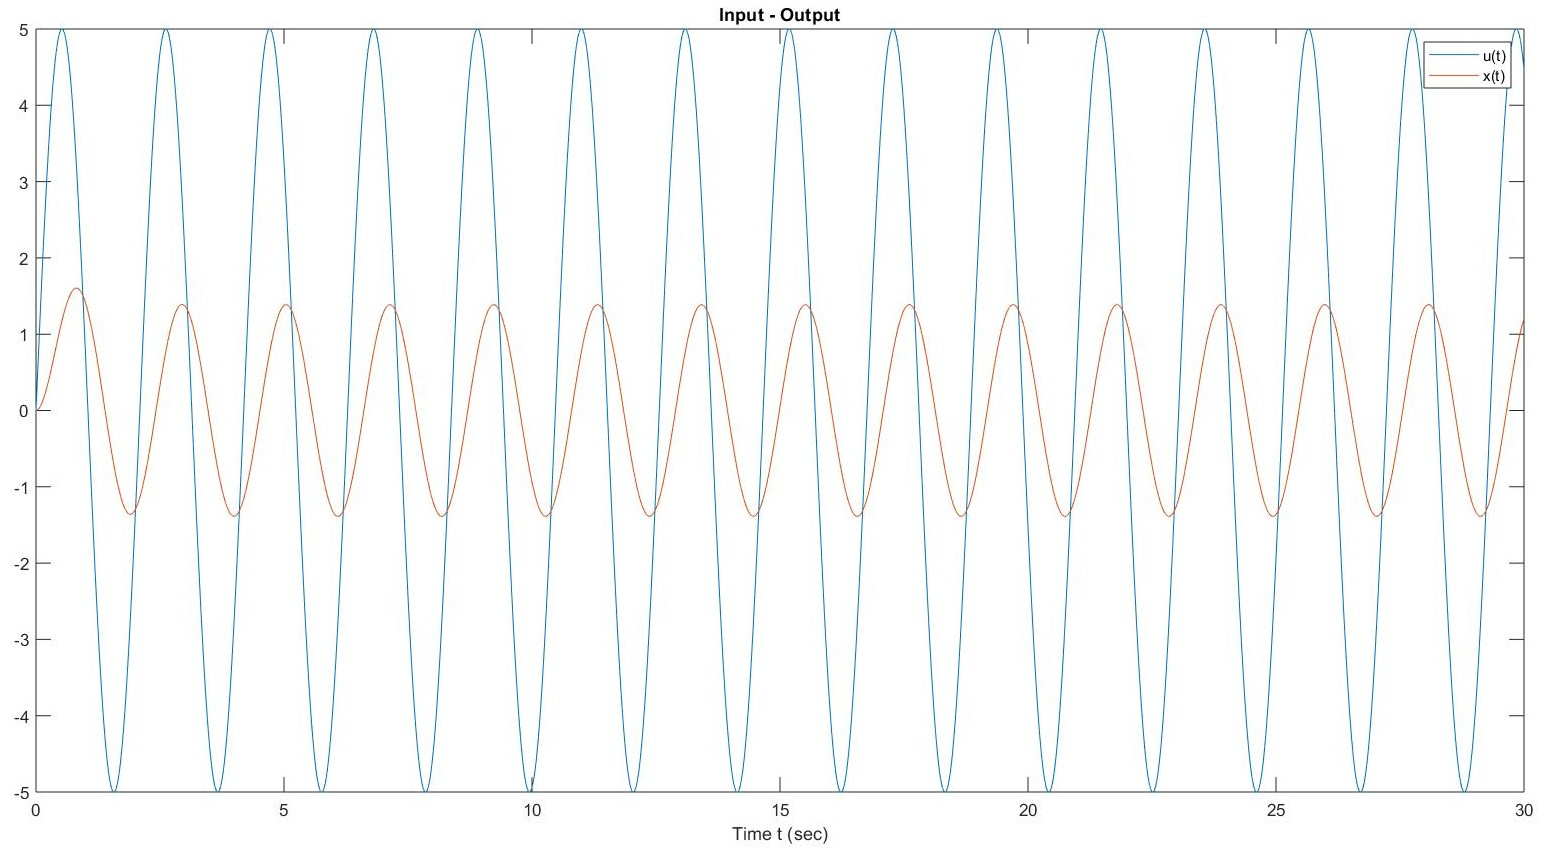
\includegraphics[width=\linewidth]{inp_out.jpg}
\centerline{Σχήμα 1: Είσοδος και Έξοδος Συστήματος}
\\ \\
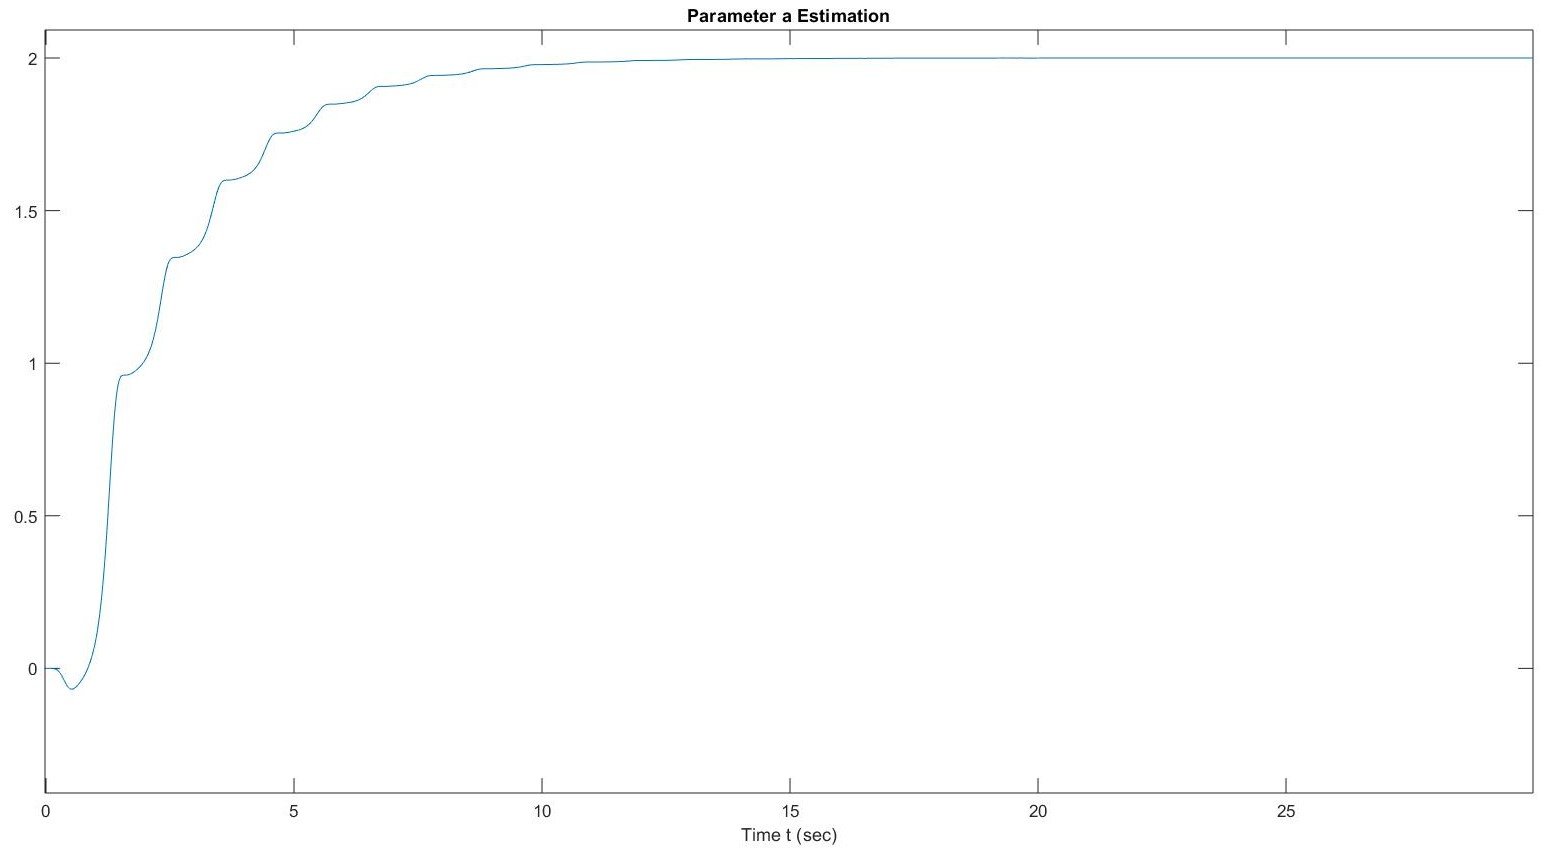
\includegraphics[width=\linewidth]{a_estim_1.jpg}
\centerline{Σχήμα 2: Εκτίμηση Παραμέτρου $\hat{a}$}
\\ \\
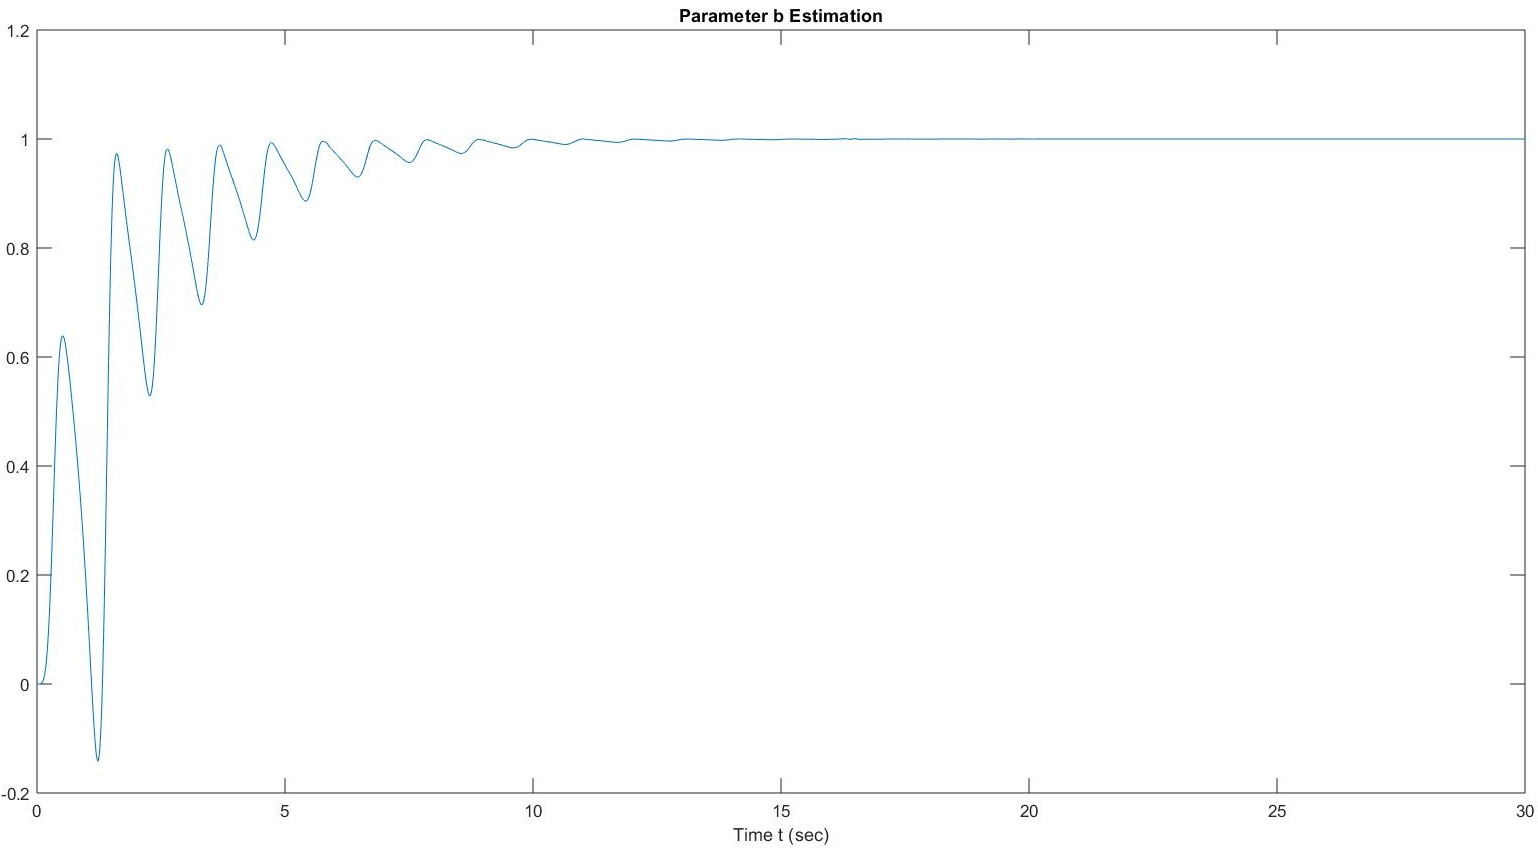
\includegraphics[width=\linewidth]{b_estim_1.jpg}
\centerline{Σχήμα 3: Εκτίμηση Παραμέτρου $\hat{b}$}
\\ \\
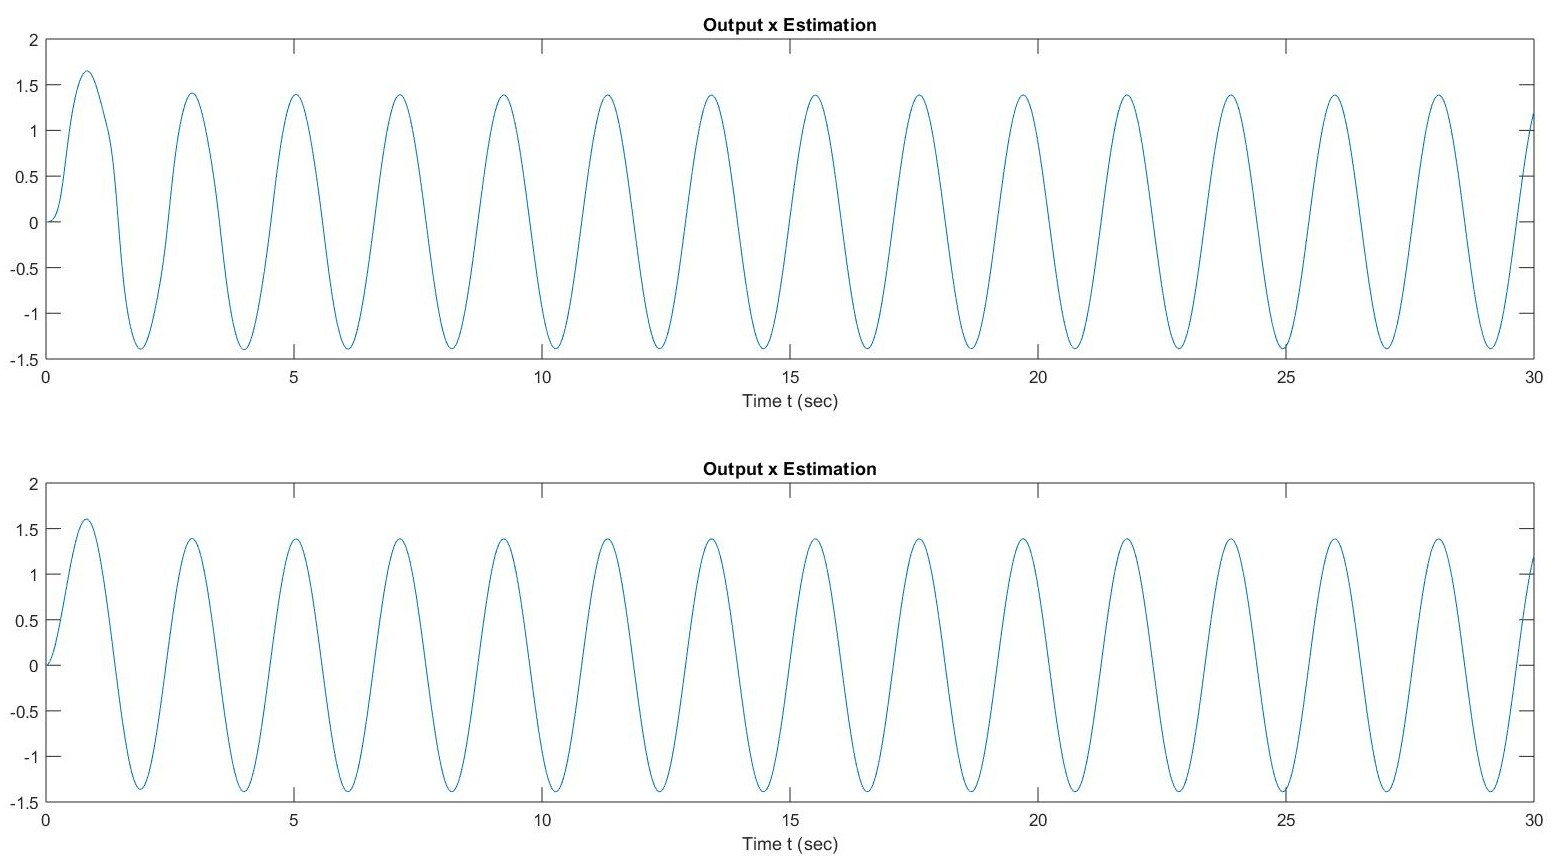
\includegraphics[width=\linewidth]{x_estim_1.jpg}
\centerline{Σχήμα 4: Εκτίμηση Κατάστασης $\hat{x}$}
\newpage
\section{Θέμα 2 }
\subsection{Θεωρητική Ανάλυση}
Για να εκτιμήσουμε τις παραμέτρους του συστήματος $(1.1)$ 
\[ \dot{x}=-ax+bu , \quad x(0)=0 \qquad \text{με }  \quad u=5sin(3t) \]
με τη χρήση εκτιμητή \textbf{παράλληλης δομής} που βασίζεται στη μέθοδο Lyapunov, θεωρούμε το σύστημα αναγνώρισης
\[ \dot{\hat{x}}=-\hat{a}\hat{x}+\hat{b}u , \quad \hat{x}(0)=0 \quad (2.2) \]
όπου με $\hat{x},\hat{a},\hat{b}$ συμβολίζονται οι εκτιμήσεις των $x,a,b$ αντίστοιχα.
\\ \\
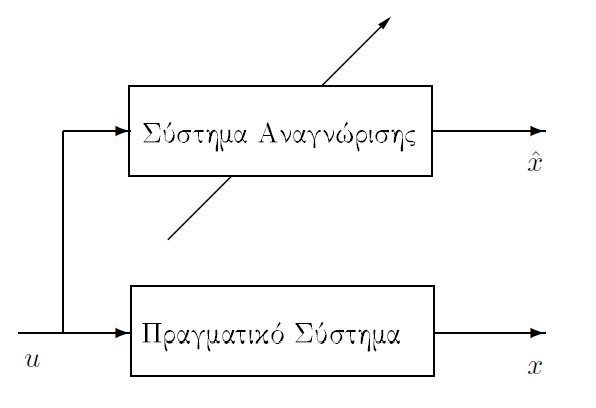
\includegraphics[width=\linewidth]{Par.jpg}
\centerline{Σχήμα 5: Διάγραμμα Βαθμίδων της Παράλληλης τοπολογίας Συστήματος Αναγνώρισης}
\\ \\ \\ \\
Στη συνέχεια θεωρούμε τη συνάρτηση σφάλματος 
\[e=x-\hat{x}\]
και από τις $(1.1),(2.2)$
\[\dot{e}=-ax+\hat{a}\hat{x}+(b-\hat{b})u  \]
επομένως προκειμένου να εξετάσουμε την ευστάθεια και τη σύγκλιση της συνάρτησης σφάλματος $e$ θεωρούμε την υποψήφια συνάρτηση Lyapunov,
\[V(e,\hat{a},\hat{b})=\frac{1}{2}e^{2}+\frac{1}{2}(\hat{a}-a)^2 + \frac{1}{2}(\hat{b}-b)^2\] η οποία είναι μη ακτινικά φραγμένη και παντού θετική εκτός από το σημείο ισορροπίας $(0,a,b)$ όπου είναι μηδέν.
Επομένως,
\[ \dot{V}=e\dot{e}+(\hat{a}-a)\dot{\hat{a}} +(\hat{b}-b)\dot{\hat{b}} \Rightarrow \]
\[\dot{V}= -eax+e\hat{a}\hat{x}+ebu-e\hat{b}u+\hat{a}\dot{\hat{a}}-a\dot{\hat{a}}+\hat{b}\dot{\hat{b}}-b\dot{\hat{b}} \Rightarrow \]
\[\dot{V}= -a(ex+\dot{\hat{a}})+\hat{a}(e\hat{x}+\dot{\hat{a}}) +b(eu-\dot{\hat{b}})-\hat{b}(eu-\dot{\hat{b}}) \Rightarrow \]
\[ \dot{V}= -a(ex+\dot{\hat{a}})+\hat{a}(e\hat{x}+\dot{\hat{a}}) +(b-\hat{b})(eu-\dot{\hat{b}})\]
\\
Στο σημείο αυτό επιλέγουμε:
\[ \dot{\hat{a}}=-e\hat{x} \quad (2.3)\]
\[\dot{\hat{b}}=eu \quad (2.4)\]
Επομένως
\[ \dot{V}= -a(ex-e\hat{x})=-ae^{2} \]
η οποία είναι αρνητικά ημιορισμένη και εξασφαλίζει την ευστάθεια της μεθόδου, ενώ ακόμα με χρήση του Λήμματος Barbalat αποδεικνύεται η ασυμπτωτική σύγκλιση των εκτιμήσεων $\hat{a},\hat{b}$ σε κάποιες σταθερές τιμές, αλλά όχι κατά ανάγκη τις πραγματικές τους τιμές $a,b$ για ομοιόμορφα φραγμένες εισόδους $u \in L_{\infty}$. Για να εξασφαλίσουμε σύγκλιση στις πραγματικές τους τιμές, ελέγχουμε την ισχύ της Συνθήκη Επιμένουσας  Διέγερσης, για κάποια $a_0,T_0 > 0 $
\[ \int_{t}^{t+T_0} u^2(\tau)d\tau \geq a_0T_0 \]
Πράγματι,
\[ \int_{t}^{t+\frac{2\pi}{3}} 25sin^2(3\tau)d\tau =\frac{25\pi}{3}=\frac{25}{2}T_0 \]
Τέλος, επιλύουμε το σύστημα των διαφορικών εξισώσεων $(1.1),(2.2),(2.3),(2.4)$ και βρίσκουμε τις εκτιμήσεις $\hat{a},\hat{b}$ που συμπίπτουν με τις πραγματικές τιμές των παραμέτρων μετά από κάποιο χρονικό διάστημα.
\\ \\
Για να εκτιμήσουμε τις παραμέτρους του συστήματος $(1.1)$ 
\[ \dot{x}=-ax+bu , \quad x(0)=0 \qquad \text{με }  \quad u=5sin(3t) \]
με τη χρήση εκτιμητή \textbf{μικτής δομής} που βασίζεται στη μέθοδο Lyapunov, θεωρούμε το σύστημα αναγνώρισης
\[ \dot{\hat{x}}=-\hat{a}\hat{x}+\hat{b}u-\theta_m(x-\hat{x}) , \quad \hat{x}(0)=0 \quad (2.5) \]
όπου με $\hat{x},\hat{a},\hat{b}$ συμβολίζονται οι εκτιμήσεις των $x,a,b$ αντίστοιχα και $\theta_m$ θετική σταθερά που επιλέγεται από εμάς.
\\
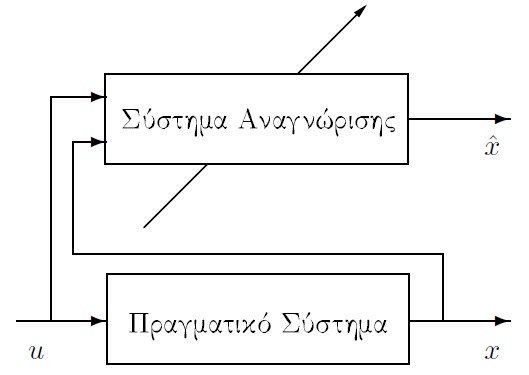
\includegraphics[width=\linewidth]{Mix.jpg}
\centerline{Σχήμα 6: Διάγραμμα Βαθμίδων της Μικτής τοπολογίας Συστήματος Αναγνώρισης}
\\ \\
Στη συνέχεια θεωρούμε τη συνάρτηση σφάλματος 
\[e=x-\hat{x}\]
και από τις $(1.1),(2.5)$
\[\dot{e}=(\theta_m-a)x-(\theta_m-\hat{a})\hat{x}+(b-\hat{b})u  \]
επομένως προκειμένου να εξετάσουμε την ευστάθεια και τη σύγκλιση της συνάρτησης σφάλματος $e$ θεωρούμε την υποψήφια συνάρτηση Lyapunov,
\[V(e,\hat{a},\hat{b})=\frac{1}{2}e^{2}+\frac{1}{2}(\hat{a}-a)^2 + \frac{1}{2}(\hat{b}-b)^2\] η οποία είναι μη ακτινικά φραγμένη και παντού θετική εκτός από το σημείο ισορροπίας $(0,a,b)$ όπου είναι μηδέν.
Επομένως,
\[ \dot{V}=e\dot{e}+(\hat{a}-a)\dot{\hat{a}} +(\hat{b}-b)\dot{\hat{b}} \Rightarrow \]
\[\dot{V}= e(\theta_m-a)x-e(\theta_m-\hat{a})\hat{x}+ebu-e\hat{b}u+\hat{a}\dot{\hat{a}}-a\dot{\hat{a}}+\hat{b}\dot{\hat{b}}-b\dot{\hat{b}} \Rightarrow \]
\[\dot{V}= e\theta_m(x-\hat{x})-a(ex+\dot{\hat{a}})+\hat{a}(e\hat{x}+\dot{\hat{a}}) +b(eu-\dot{\hat{b}})-\hat{b}(eu-\dot{\hat{b}}) \Rightarrow \]
\[ \dot{V}=e^2\theta_m -a(ex+\dot{\hat{a}})+\hat{a}(e\hat{x}+\dot{\hat{a}}) +(b-\hat{b})(eu-\dot{\hat{b}})\]
\\
Στο σημείο αυτό επιλέγουμε:
\[ \dot{\hat{a}}=-ex \quad (2.6)\]
\[\dot{\hat{b}}=eu \quad (2.7)\]
Επομένως
\[ \dot{V}= e^2\theta_m+\hat{a}(e\hat{x}-ex)=-e^{2}(\hat{a}-\theta_m) \]
η οποία είναι αρνητικά ημιορισμένη όταν $\hat{a}\geq\theta_m$ και εξασφαλίζει την ευστάθεια της μεθόδου, ενώ ακόμα με χρήση του Λήμματος Barbalat αποδεικνύεται η ασυμπτωτική σύγκλιση των εκτιμήσεων $\hat{a},\hat{b}$ σε κάποιες σταθερές τιμές, αλλά όχι κατά ανάγκη τις πραγματικές τους τιμές $a,b$ για ομοιόμορφα φραγμένες εισόδους $u \in L_{\infty}$. Για να εξασφαλίσουμε σύγκλιση στις πραγματικές τους τιμές, ελέγχουμε την ισχύ της Συνθήκη Επιμένουσας Διέγερσης, για κάποια $a_0,T_0 > 0 $
\[ \int_{t}^{t+T_0} u^2(\tau)d\tau  \geq a_0T_0 \]
Πράγματι,
\[ \int_{t}^{t+\frac{2\pi}{3}} 25sin^2(3\tau)d\tau =\frac{25\pi}{3}=\frac{25}{2}T_0 \]
\\ \\
Η επιλογή του $\theta_m$ είναι επιθυμητό να πάρει μια τιμή αρκετά μικρή ώστε η ταχύτητα σύγκλισης να είναι η κατά το δυνατόν μεγαλύτερη, όπως φαίνεται από την $\dot{V}$\quad ($\hat{a}-\theta_m \gg 0$). Έτσι επιλέγουμε τελικά $\theta_m=0.01$. \\
Παρατηρούμε, επίσης, ότι αν το $\theta_m$ είναι μηδέν έχουμε ουσιαστικά την περίπτωση της παράλληλης δομής.
\\ \\
Τέλος, επιλύουμε το σύστημα των διαφορικών εξισώσεων $(1.1),(2.5),(2.6),(2.7)$ και βρίσκουμε τις εκτιμήσεις $\hat{a},\hat{b}$ που συμπίπτουν με τις πραγματικές τιμές των παραμέτρων μετά από κάποιο χρονικό διάστημα.
\\ \\
Σε περίπτωση εμφάνισης θορύβου στις μετρήσεις της κατάστασης του συστήματος, που περιγράφεται από τη συνάρτηση 
$ \eta (t)=\eta_{0} sin(2 \pi ft),$ $\eta_{0}=0.15,$ $f=20Hz$, περιμένουμε με τη χρήση της παράλληλης δομής η επίδραση του θορύβου να είναι λιγότερο έντονη σε σχέση με αυτήν στη μικτή δομή. Αυτό συμβαίνει διότι στη μεικτή δομή εκμεταλλευόμαστε την έξοδο του συστήματος για τη λειτουργία του συστήματος αναγνώρισης κάτι που δεν συμβαίνει στην παράλληλη δομή. Έτσι, τυχόν σφάλματα στις μετρήσεις καθιστούν την εκτίμηση των παραμέτρων περισσότερο ανακριβή.
\\ \\
Κατά την εκτέλεση της εργασίας χρησιμοποιήθηκε $\theta_m=0.01$ για χρόνους από $t=0$ μέχρι $t=30 sec$ με βήμα $0.0001 sec$
\subsection{Αρχεία και Αποτελέσματα Matlab}
Το δεύτερο θέμα αποτελείται από πέντε αρχεία, τα $erwtimaB.m$, $dx\_ mixdt.m$, $dx\_ pardt.m$ , $dx\_ mixNoisedt.m$ , $dx\_ parNoisedt.m$. Για την εκτέλεση του  κώδικα τρέχουμε το αρχείο $erwtimaB.m$.
\\ \\
Στο αρχείο $erwtimaB.m$ επιλύονται τα συστημάτα των διαφορικών εξισώσεων $(1.1),(2.2),(2.3),(2.4)$ και $(1.1),(2.5),(2.6),(2.7)$ με χρήση της συνάρτησης του $Matlab$, $ode45$, για την περίπτωση της παράλληλης και μικτής δομής αντίστοιχα και στη συνέχεια υπολογίζεται η συνάρτηση των εκτιμήσεων με το χρόνο. Κατόπιν, επιλύονται τα ίδια συστήματα ξανά, με την παρουσία θορύβου στη μέτρηση της κατάστασης $x$ και παράγονται τα αντίστοιχα διαγράμματα.
\\ \\
Στα αρχεία $dx\_ pardt.m$, $dx\_ parNoisedt.m$ περιέχεται το σύστημα των τεσσάρων διαφορικών εξισώσεων για την περίπτωση παράλληλης δομής όταν δεν υπάρχει και όταν υπάρχει θόρυβος αντίστοιχα, ενώ στα αρχεία $dx\_ mixdt.m$, $dx\_ mixNoisedt.m$ περιέχεται το σύστημα των τεσσάρων διαφορικών εξισώσεων για την περίπτωση μικτής δομής όταν δεν υπάρχει και όταν υπάρχει θόρυβος αντίστοιχα.
\\ \\
Οι γραφικές παραστάσεις των εκτιμήσεων των παραμέτρων $\hat{a},\hat{b}$, καθώς επίσης και της κατάστασης $\hat{x}$ όταν δεν εμφανίζεται και όταν εμφανίζεται θόρυβος φαίνονται αντίστοιχα στα Σχήματα 7-18.
\\ \\
\includegraphics[width=\linewidth]{a_estim_par_2.jpg}
\centerline{Σχήμα 7: Εκτίμηση Παραμέτρου $\hat{a}$ - Παράλληλη Δομή}
\\ \\
\includegraphics[width=\linewidth]{b_estim_par_2.jpg}
\centerline{Σχήμα 8: Εκτίμηση Παραμέτρου $\hat{b}$ - Παράλληλη Δομή}
\\ \\
\includegraphics[width=\linewidth]{x_estim_par_2.jpg}
\centerline{Σχήμα 9: Εκτίμηση Κατάστασης $\hat{x}$ - Παράλληλη Δομή}
\\ \\
\includegraphics[width=\linewidth]{a_estim_mix_2.jpg}
\centerline{Σχήμα 10: Εκτίμηση Παραμέτρου $\hat{a}$ - Μικτή Δομή}
\\ \\
\includegraphics[width=\linewidth]{b_estim_mix_2.jpg}
\centerline{Σχήμα 11: Εκτίμηση Παραμέτρου $\hat{b}$ - Μικτή Δομή}
\\ \\
\includegraphics[width=\linewidth]{x_estim_mix_2.jpg}
\centerline{Σχήμα 12: Εκτίμηση Κατάστασης $\hat{x}$ - Μικτή Δομή}
\\ \\
Για το θόρυβο, όπως βλέπουμε από τα Σχήματα 13-18, λόγω του ότι το πλάτος είναι μικρό, δεν παρουσιάζεται μεγάλη διαφορά μεταξύ των δύο Δομών. Ωστόσο, αν αυξήσουμε το πλάτος $\eta_0$ μπορούμε να παρατηρήσουμε μεγαλύτερη επίδραση πάνω στο σύστημα αναγνώρισης μικτής δομής όπως αναφέρθηκε προηγουμένως. Αντιθέτως μεταβάλλοντας τη συχνότητα οι αλλαγές δεν είναι τόσο αισθητές, απλώς η συνάρτηση δεν αποσβαίνει  τόσο ομαλά όταν αυτή είναι υψηλή.
\\
\includegraphics[width=\linewidth]{a_estim_par_Noise_2.jpg}
\centerline{Σχήμα 13: Εκτίμηση Παραμέτρου $\hat{a}$ - Παράλληλη Δομή με Θόρυβο $\eta$}
\\ \\
\includegraphics[width=\linewidth]{b_estim_par_Noise_2.jpg}
\centerline{Σχήμα 14: Εκτίμηση Παραμέτρου $\hat{b}$ - Παράλληλη Δομή με Θόρυβο $\eta$}
\\ \\
\includegraphics[width=\linewidth]{x_estim_par_Noise_2.jpg}
\centerline{Σχήμα 15: Εκτίμηση Κατάστασης $\hat{x}$ - Παράλληλη Δομή με Θόρυβο $\eta$}
\\ \\
\includegraphics[width=\linewidth]{a_estim_mix_Noise_2.jpg}
\centerline{Σχήμα 16: Εκτίμηση Παραμέτρου $\hat{a}$ - Μικτή Δομή με Θόρυβο $\eta$}
\\ \\
\includegraphics[width=\linewidth]{b_estim_mix_Noise_2.jpg}
\centerline{Σχήμα 17: Εκτίμηση Παραμέτρου $\hat{b}$ - Μικτή Δομή με Θόρυβο $\eta$}
\\ \\
\includegraphics[width=\linewidth]{x_estim_mix_Noise_2.jpg}
\centerline{Σχήμα 18: Εκτίμηση Κατάστασης $\hat{x}$ - Μικτή Δομή με Θόρυβο $\eta$}
\\
\newpage
\section{Θέμα 3}
\subsection{Θεωρητική Ανάλυση}
Θέλουμε να εκτιμήσουμε τις παραμέτρους του συστήματος
\[\dot{x}= Ax+Bu \qquad x(0,0)=\begin{bmatrix}   
			0\\
			0
\end{bmatrix} \quad(3.1)\]
με $u=10sin(2t)+5sin(7.5t)$, $ $ χρησιμοποιώντας έναν εκτιμητή πραγματικού χρόνου παράλληλης δομής. Θεωρούμε, λοιπόν, το σύστημα αναγνώρισης
\[ \dot{\hat{x}}=\hat{A}\hat{x}+\hat{B}u , \quad \hat{x}(0,0)=\begin{bmatrix}   
			0\\
			0
\end{bmatrix} \quad (3.2) \]
όπου με $\hat{x},\hat{A},\hat{B}$ συμβολίζονται οι εκτιμήσεις των $x,A,B$ αντίστοιχα, με \\
\[ Α= \begin{bmatrix}   
			a_{11} & a_{12} \\
			a_{21} & a_{22}
\end{bmatrix}= \begin{bmatrix}   
			-0.25 & 3 \\
			-5 & -1
\end{bmatrix} 
\qquad
B=\begin{bmatrix}   
			b_{1}\\
			b_{2}
\end{bmatrix}=
\begin{bmatrix}   
			1\\
			2.2
\end{bmatrix}
\]
Ακολουθώντας αντίστοιχη διαδικασία με αυτή του Θέματος 2, θεωρούμε τη διανυσματική συνάρτηση σφάλματος $e=x-\hat{x}$ και την υποψήφια συνάρτηση $Laypunov$,
\[V=\frac{1}{2}ee^{T}+\frac{1}{2}tr\{(\hat{A}-A)(\hat{A}-A)^{T}\}+\frac{1}{2}tr\{(\hat{B}-B)(\hat{B}-B)^{T}\} \]
Για το σφάλμα $e$ από τις $(3.1),(3.2)$ ισχύει
\[ \dot{e}=\dot{x}-\dot{\hat{x}}= Ax-\hat{A}\hat{x}-(\hat{B}-B)u\]
\\
Έτσι, μετά από πράξεις καταλήγουμε ότι $\dot{V}=eAe^{T}<0$, όταν έχουμε επιλέξει
\[ \dot{A}=e^{T}\hat{x} \quad (3.3) \] 
\[\dot{B}=e^{T}u \quad (3.4) \]
δεδομένου ότι ο $A$ είναι αρνητικά ημιορισμένος (ή αρνητικά ορισμένος όπως στην προκειμένη περίπτωση αφού $a_{11}=-0.25<0$ και $det(A)=15.25>0$) και η είσοδος $u$ φραγμένη, $u\in L_{\infty}$. Επομένως, εξασφαλίζεται η ευστάθεια της μεθόδου, ενώ ακόμα με χρήση του Λήμματος Barbalat αποδεικνύεται η ασυμπτωτική σύγκλιση των εκτιμήσεων $\hat{A},\hat{B}$  σε κάποιες σταθερές τιμές, αλλά όχι κατά ανάγκη τις πραγματικές τους τιμές. Για να εξασφαλίσουμε σύγκλιση στις πραγματικές τους τιμές, ελέγχουμε την ισχύ της Συνθήκη Επιμένουσας Διέγερσης, για κάποια $a_0,T_0 > 0 $
\[ \int_{t}^{t+T_0} u^2(\tau)d\tau \geq a_0T_0 \]
Πράγματι,
\[ \int_{t}^{t+4\pi} \left[10sin(2\tau)+5sin(7.5\tau)\right]^2 d\tau =250 \pi =\frac{125}{2}T_0 \]
Τέλος, επιλύουμε το σύστημα των διαφορικών εξισώσεων $(3.1),(3.2),(3.3),(3.4)$ και βρίσκουμε τις εκτιμήσεις $\hat{A},\hat{B}$. Ωστόσο στην περίπτωση αυτή, από το σύστημα αυτό προκύπτουν δέκα διαφορικές εξισώσεις δεδομένου ότι το $x$ είναι πλέον διανυσματικό μέγεθος και όχι βαθμωτό, ενώ η είσοδος $u$ είναι βαθμωτή. Συγκεκριμένα από τις παραπάνω σχέσεις αντίστοιχα, έχουμε:
\[ \dot{x_1}=a_{11}x_1+a_{12}x_2+b_1u \]
\[ \dot{x_2}=a_{21}x_1+a_{22}x_2+b_2u \]
\\
\[ \dot{\hat{x_1}}=\hat{a_{11}}\hat{x_1}+\hat{a_{12}}\hat{x_2}+\hat{b_1}u \]
\[ \dot{\hat{x_2}}=\hat{a_{21}}\hat{x_1}+\hat{a_{22}}\hat{x_2}+\hat{b_2}u \]
\\
\[ \dot{\hat{a_{11}}}=\hat{x_1}(x_1-\hat{x_1}) \]
\[ \dot{\hat{a_{12}}}=\hat{x_2}(x_1-\hat{x_1}) \]
\[ \dot{\hat{a_{21}}}=\hat{x_1}(x_2-\hat{x_2}) \]
\[ \dot{\hat{a_{22}}}=\hat{x_2}(x_2-\hat{x_2}) \]
\\
\[ \dot{\hat{b_{1}}}=u(x_1-\hat{x_1}) \]
\[ \dot{\hat{b_{2}}}=u(x_2-\hat{x_2}) \] 
\\
Για την εκτέλεση της εργασίας χρησιμοποιήθηκε βήμα $0.0001 sec$ για χρόνους από $t=0$ μέχρι $t=60 sec$. 
\subsection{Αρχεία και Αποτελέσματα Matlab}
Το τρίτο θέμα αποτελείται από δύο αρχεία, τα $erwtimaC.m$ και $dx\_ dt.m$. Για την εκτέλεση του  κώδικα τρέχουμε το αρχείο $erwtimaC.m$.
\\ \\
Στο αρχείο $erwtimaC.m$ επιλύεται το σύστημα των διαφορικών εξισώσεων $(3.1)-(3.4)$ με χρήση της συνάρτησης του $Matlab$, $ode45$, και στη συνέχεια παράγονται τα διαγράμματα με τις χρονικές αποκρίσεις των εκτιμήσεων $\hat{A},\hat{B}$ καθώς επίσης και του συστήματος αναγνώρισης $\hat{x}$.
\\ \\
Στο αρχείο $dx\_ dt.m$ περιέχεται το σύστημα των δέκα διαφορικών εξισώσεων.
\\
Οι γραφικές παραστάσεις της εξόδου,του συστήματος αναγνώρισης παράλληλης δομής $\hat{x}$ καθώς και των εκτιμήσεων $\hat{A},\hat{B}$ φαίνονται στα Σχήματα 19 έως 26 αντίστοιχα.
\\ \\
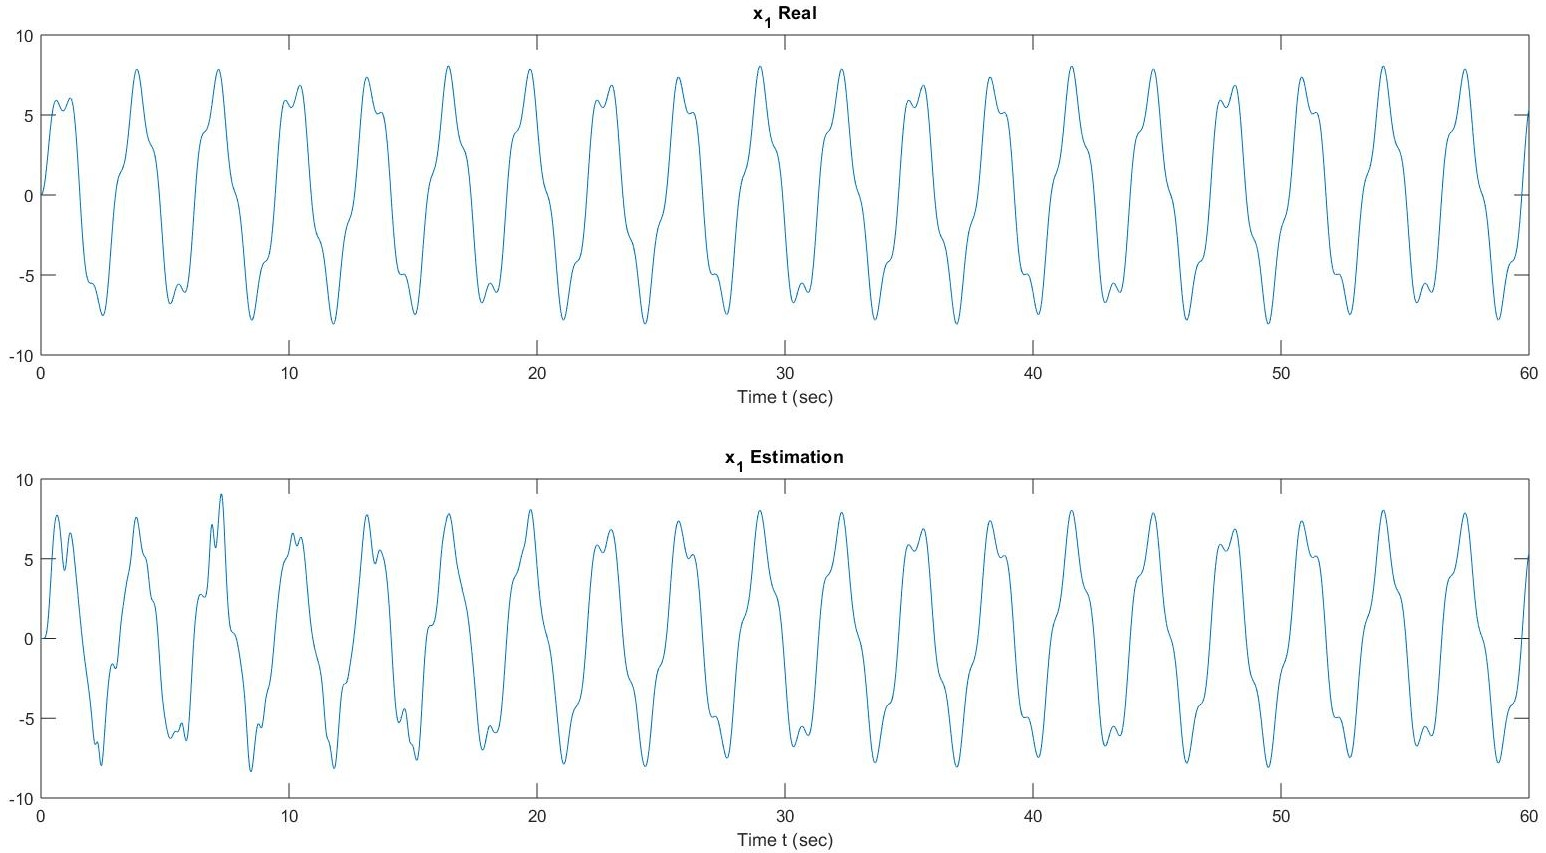
\includegraphics[width=\linewidth]{x1_estim_3.jpg}
\centerline{Σχήμα 19: Κατάσταση και Εκτίμηση Κατάστασης $\hat{x_1}$ - Παράλληλη Δομή}
\\ \\
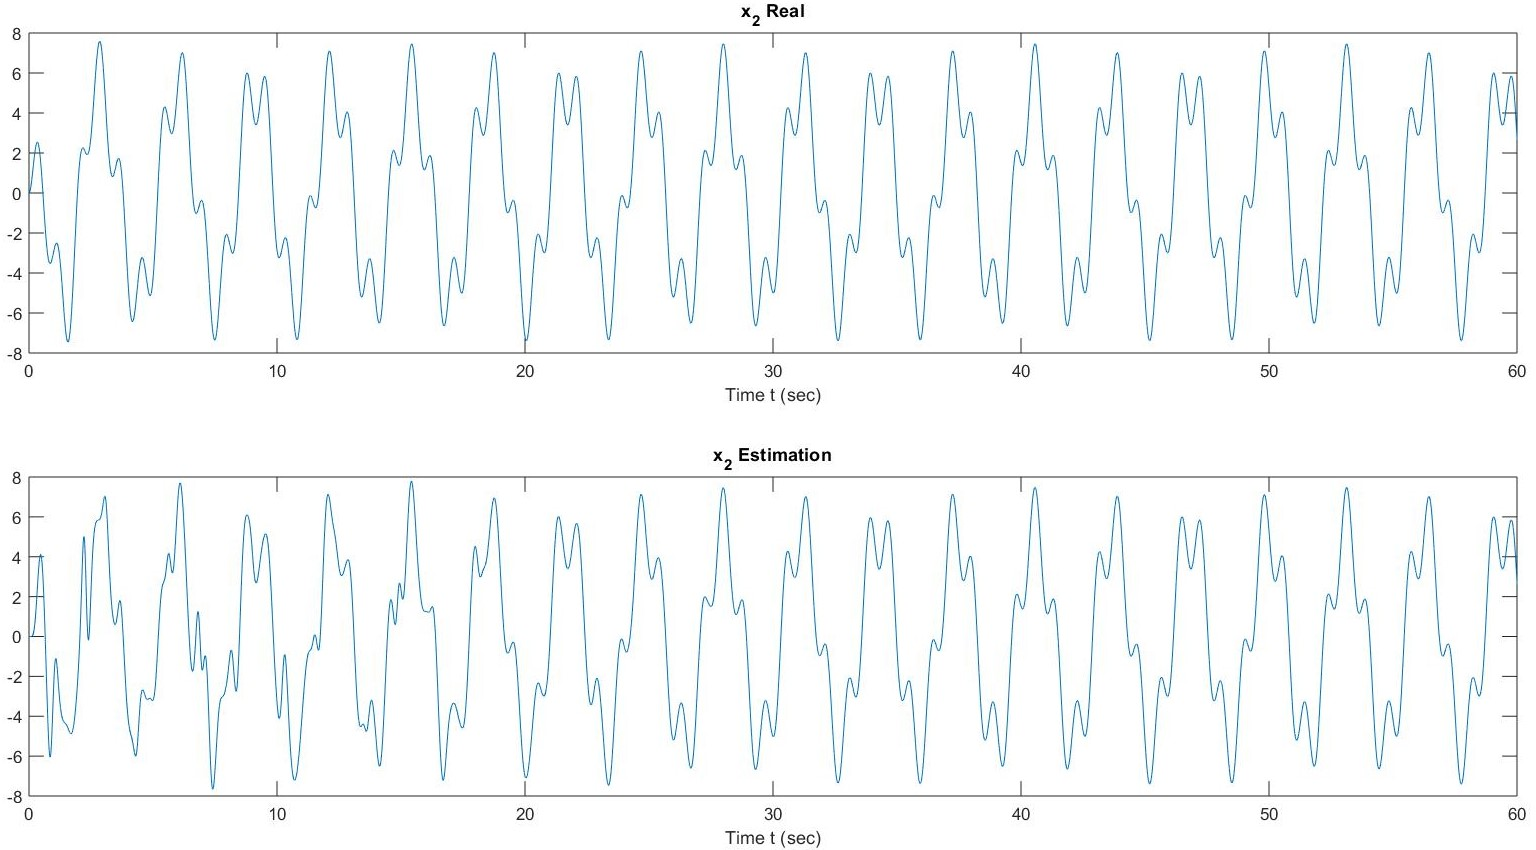
\includegraphics[width=\linewidth]{x2_estim_3.jpg}
\centerline{Σχήμα 20: Κατάσταση και Εκτίμηση Κατάστασης $\hat{x_2}$ - Παράλληλη Δομή}
\\ \\
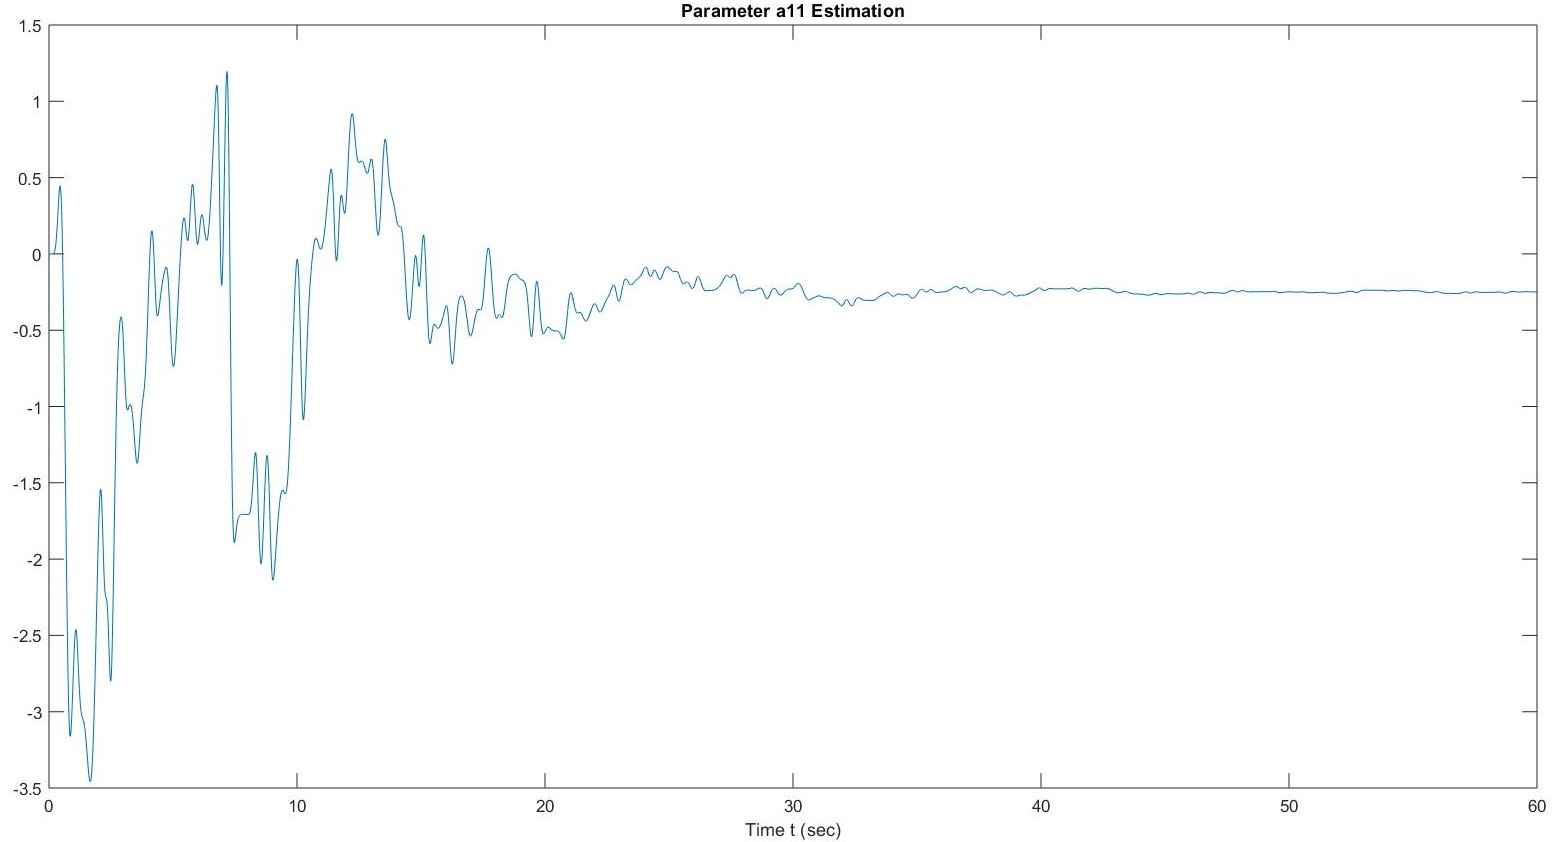
\includegraphics[width=\linewidth]{a11_estim_3.jpg}
\centerline{Σχήμα 21: Εκτίμηση Παραμέτρου $\hat{a_{11}}$ - Παράλληλη Δομή}
\\ \\
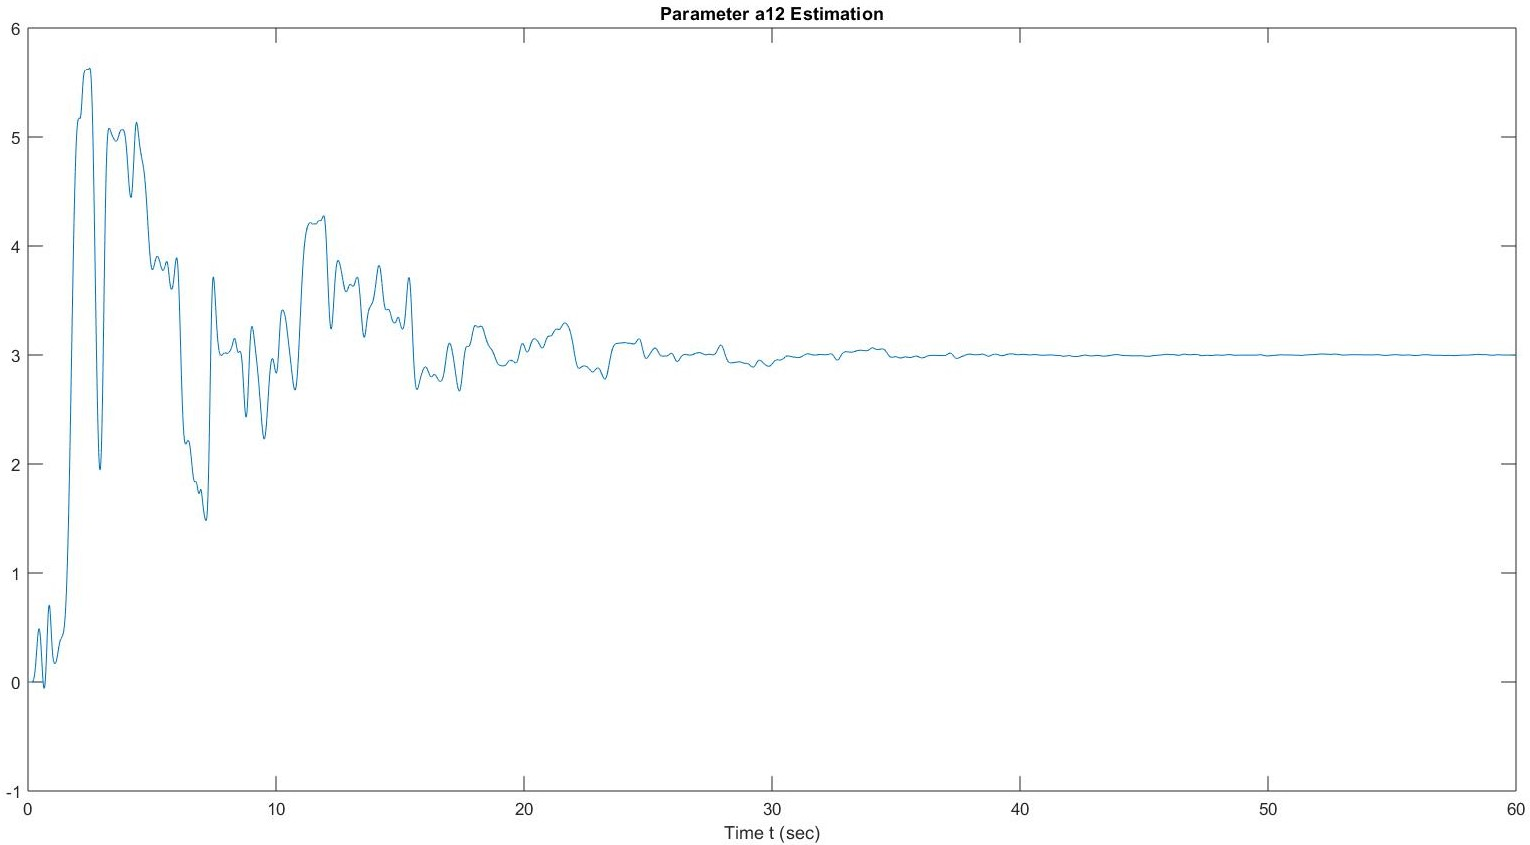
\includegraphics[width=\linewidth]{a12_estim_3.jpg}
\centerline{Σχήμα 22: Εκτίμηση Παραμέτρου $\hat{a_{12}}$ - Παράλληλη Δομή}
\\ \\
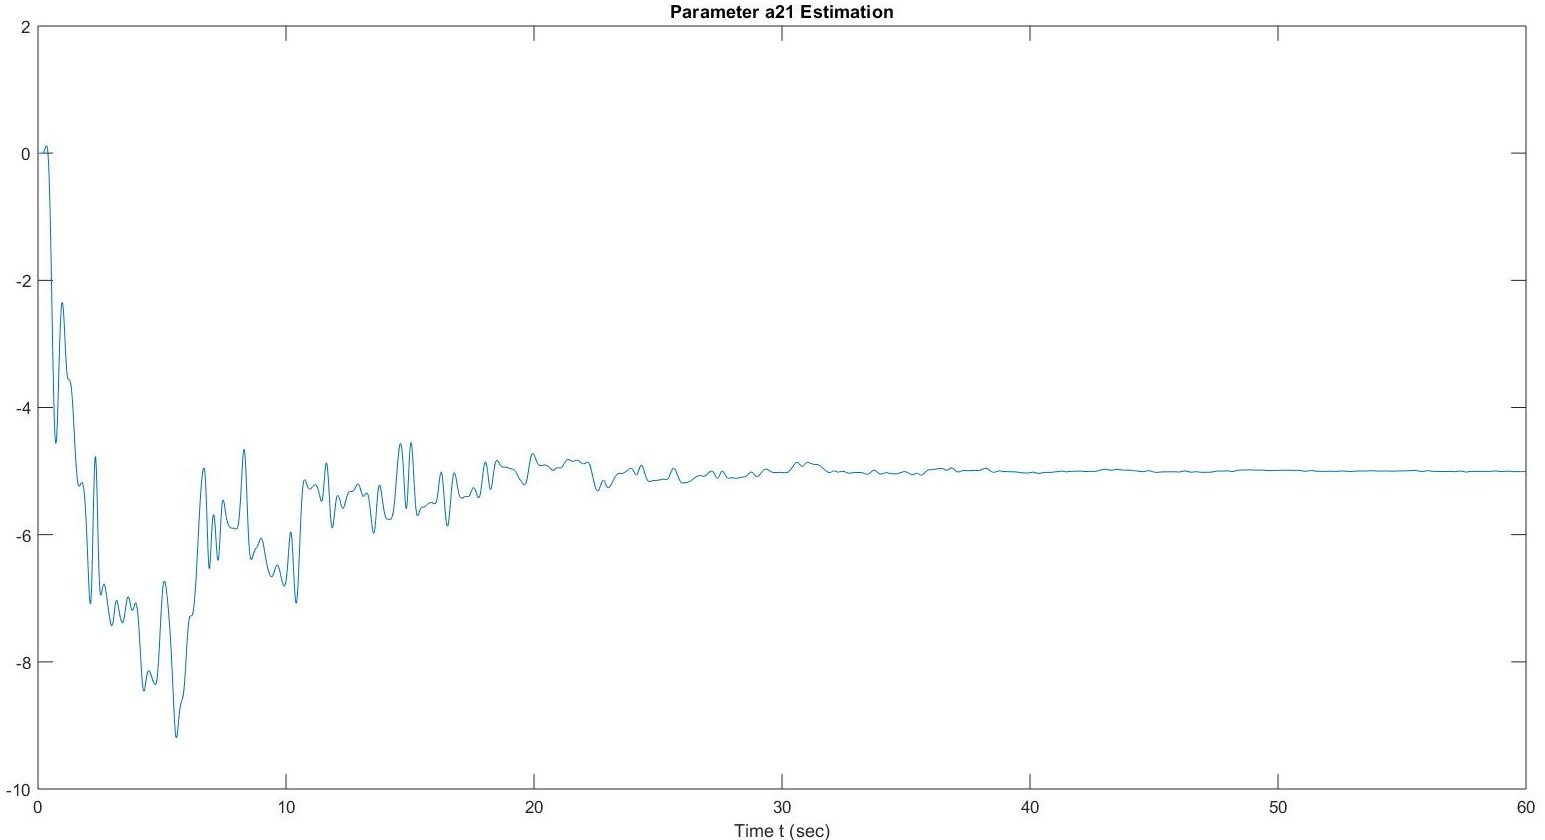
\includegraphics[width=\linewidth]{a21_estim_3.jpg}
\centerline{Σχήμα 23: Εκτίμηση Παραμέτρου $\hat{a_{21}}$ - Παράλληλη Δομή}
\\ \\
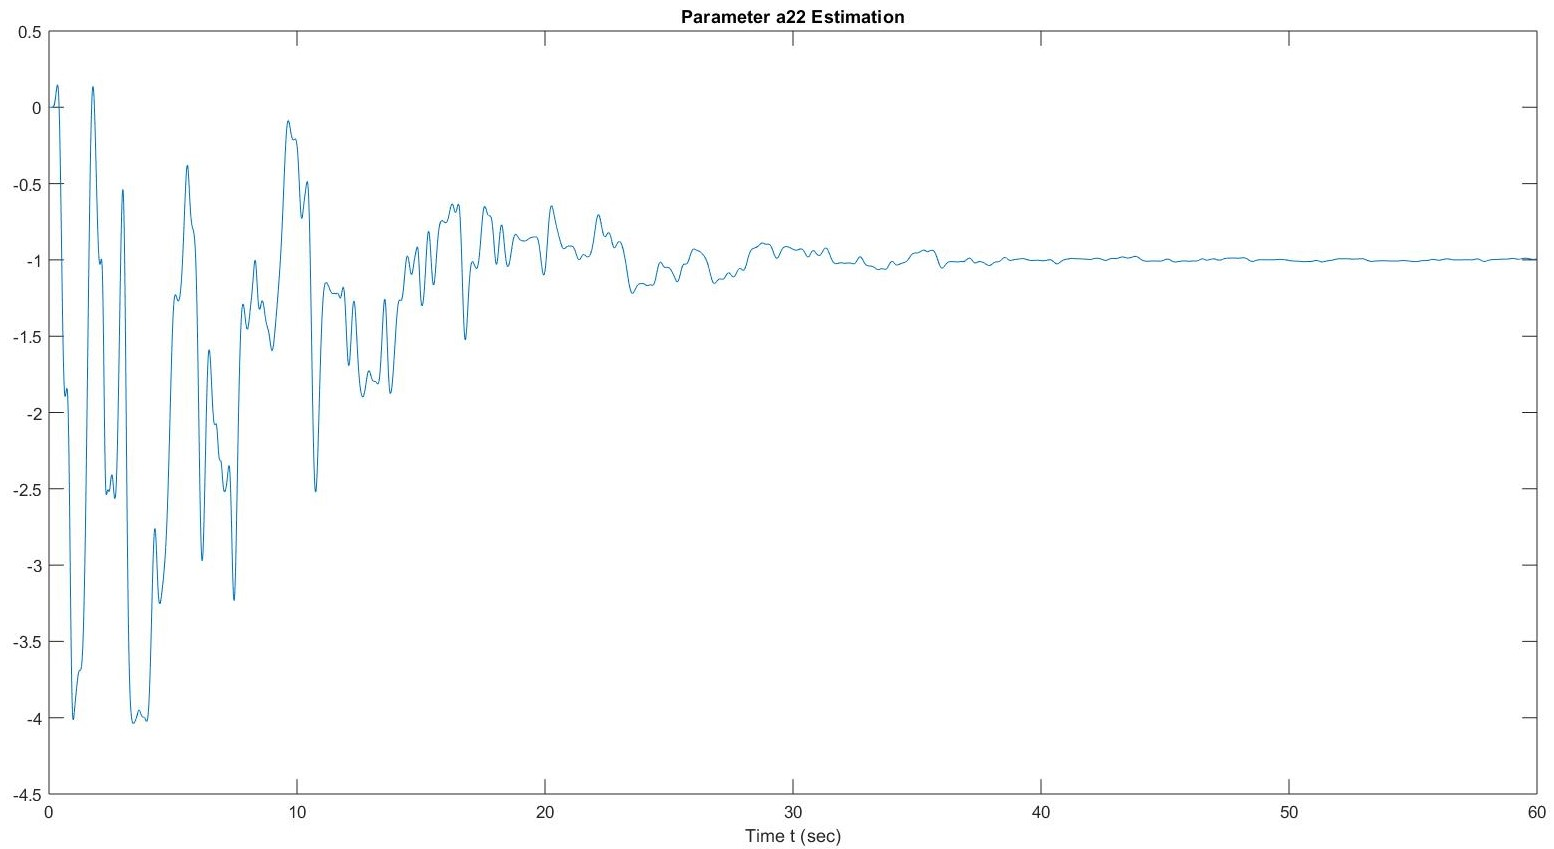
\includegraphics[width=\linewidth]{a22_estim_3.jpg}
\centerline{Σχήμα 24: Εκτίμηση Παραμέτρου $\hat{a_{22}}$ - Παράλληλη Δομή}
\\ \\
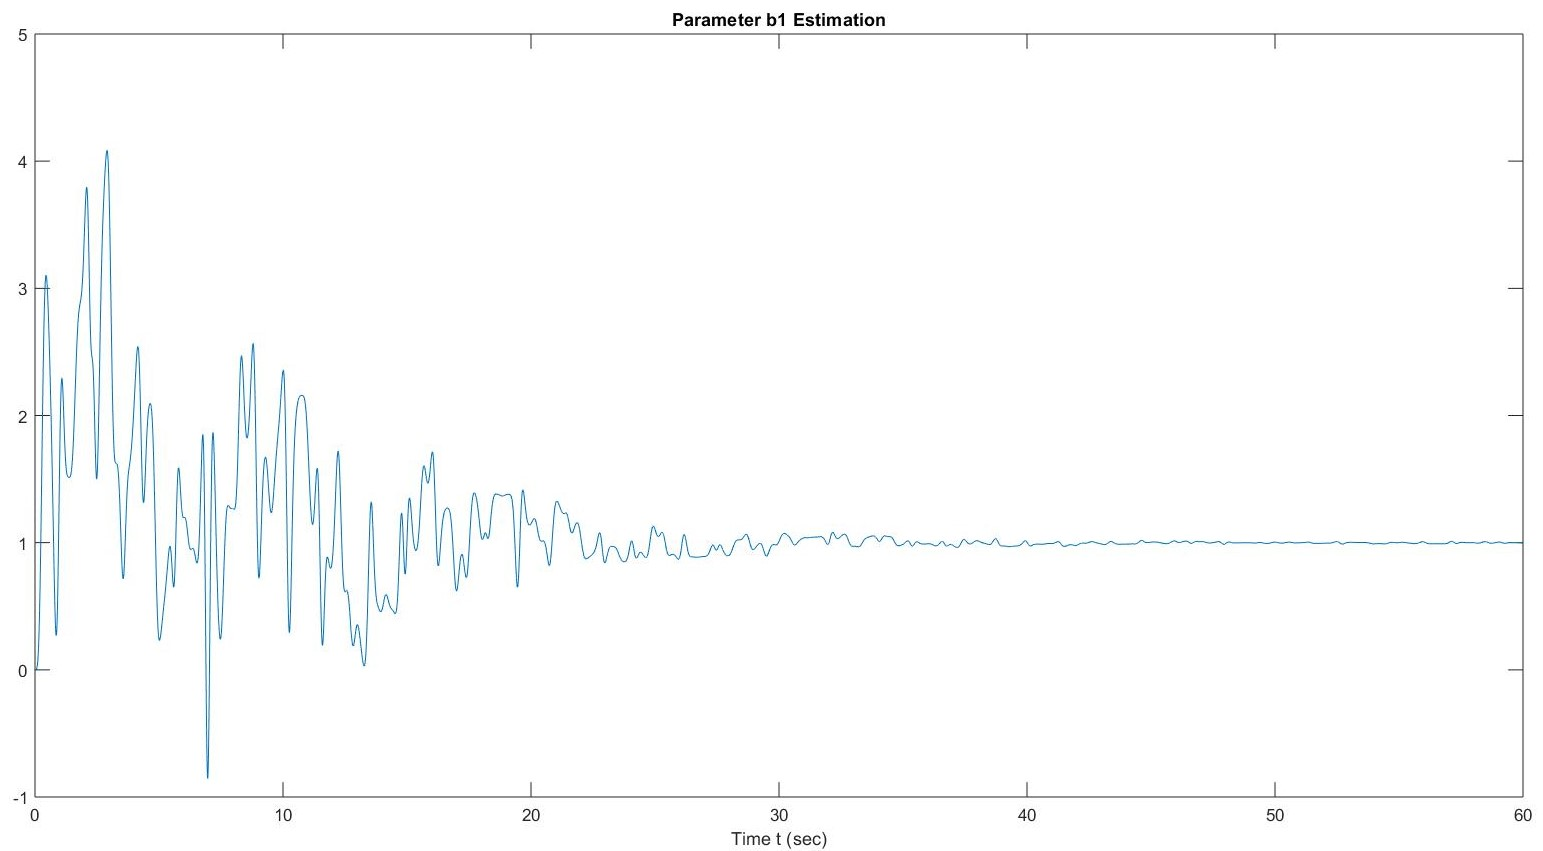
\includegraphics[width=\linewidth]{b1_estim_3.jpg}
\centerline{Σχήμα 25: Εκτίμηση Παραμέτρου $\hat{b_1}$ - Παράλληλη Δομή}
\\ \\
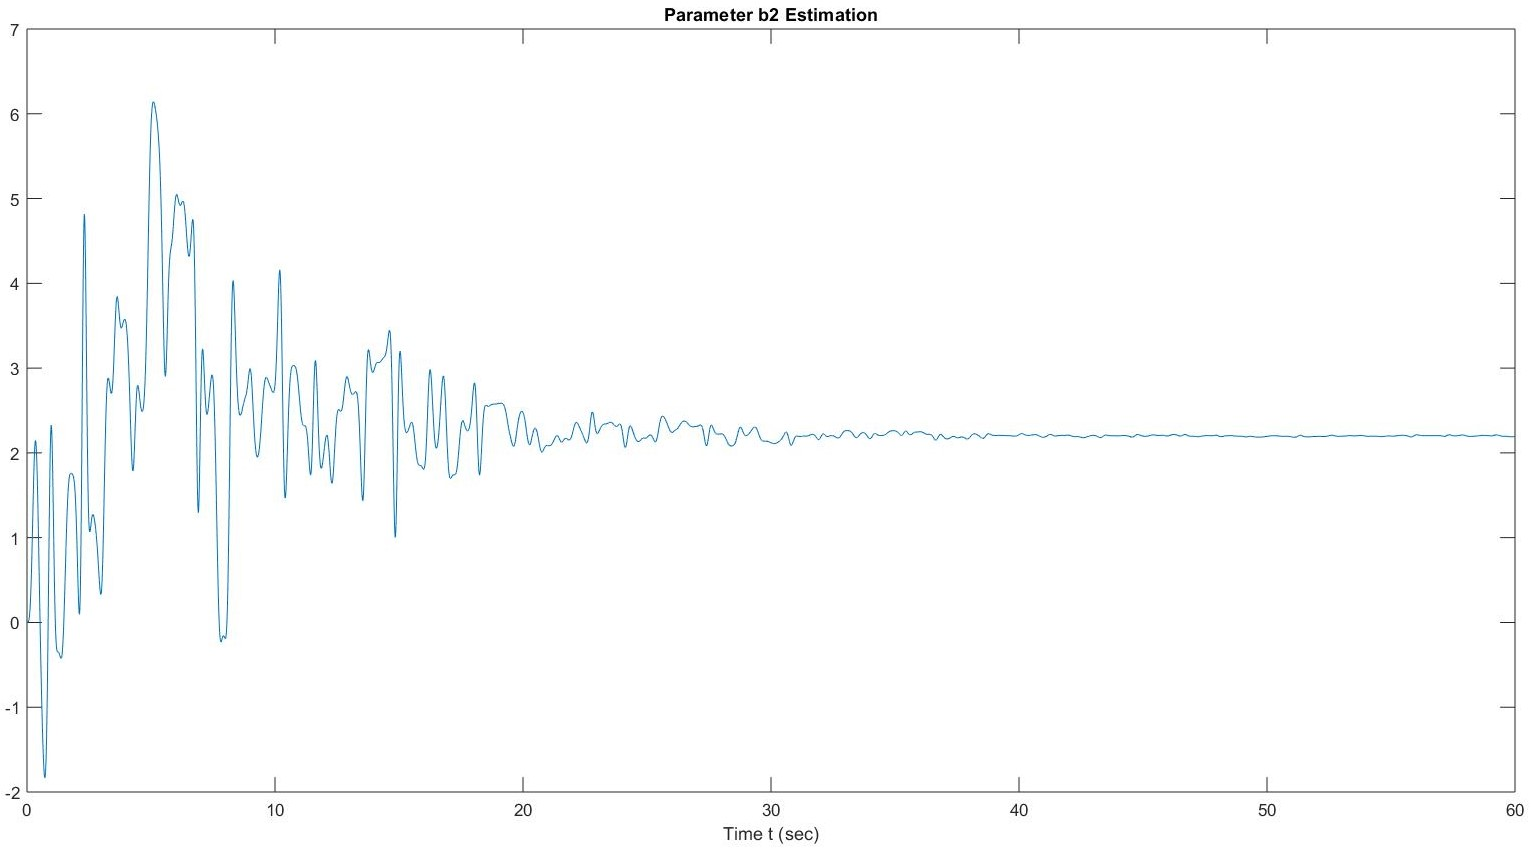
\includegraphics[width=\linewidth]{b2_estim_3.jpg}
\centerline{Σχήμα 26: Εκτίμηση Παραμέτρου $\hat{b_2}$ - Παράλληλη Δομή}
\\ \\ \\
Πράγματι, οι εκτιμήσεις συγκλίνουν τελικά στις πραγματικές τιμές των παραμέτρων μετά από περίπου 40sec.
\end{document}